\documentclass[letterpaper,journal]{IEEEtran}
\usepackage{amsmath,amssymb,amsfonts}
\usepackage{graphicx}
\usepackage{booktabs,array,tabularx}
\usepackage{cite}
\usepackage{xcolor}
\usepackage{tikz}
\usetikzlibrary{arrows.meta,positioning,fit}
\usepackage[hidelinks]{hyperref}
\newcommand{\pending}{\textit{TBD}}
\newcommand{\mr}{\textnormal{\textsc{MemoryReset5}}}
\newcommand{\rmodes}{\textnormal{\textsc{RealModes3}}}
\newcommand{\R}{\mathbb{R}}
\DeclareMathOperator{\diag}{diag}
\DeclareMathOperator{\spec}{spec}
\DeclareMathOperator{\Acc}{Acc}
\newtheorem{proposition}{Proposition}
\hyphenation{multi-compartment re-parameterization}
\begin{document}

\title{SPRiF: Spectral Memory and Scalar Reset for Spiking Neurons}
\author{\textit{Author information to be completed}}
\maketitle

\begin{abstract}
Temporal processing in spiking neural networks requires neurons to retain input history while repeatedly generating spikes. When a membrane carries both functions, reset enters the same recurrence as the stored history. We present SPRiF, a five-state neuron that couples a constrained spectral memory and an auxiliary linear filter to a scalar resettable membrane. The spectral block contains one real decay mode and a damped rotational pair. Two learned readouts provide a direct membrane drive and a filtered drive with a one-step delay. A spike subtracts one fixed threshold from the membrane and leaves the four memory and filter coordinates unchanged by direct local reset. The parameterization uses eleven trainable dynamics coefficients per neuron. We derive the spectral and effective drive kernels, establish controllability of the three-dimensional spectral block, and prove boundedness of the local states for bounded current. We also specify the reset identity and its boundary under recurrent feedback. The empirical protocol covers five temporal classification benchmarks, two controls with matched state and coefficient counts, and a recurrent spike-intervention task. Measurements for this parameterization are pending; the available historical results are identified separately.
\end{abstract}

\begin{IEEEkeywords}
Spiking neural networks, temporal processing, spectral memory, neuron dynamics, scalar reset.
\end{IEEEkeywords}

\section{Introduction}
\label{sec:introduction}

\IEEEPARstart{S}{piking} neural networks (SNNs) process temporal signals through stateful neurons and discrete output events. In sequence classification, a neuron must combine recent evidence with context accumulated much earlier. Its temporal representation must remain useful while the network continues to emit spikes. The way state variables carry memory and respond to each spike is therefore part of the computational design.

A leaky integrate-and-fire (LIF) neuron uses a scalar membrane to accumulate current, determine firing, and receive reset. Unrolling its recurrence exposes both input history and reset history in the same decaying trace. This arrangement is compact, but it ties the retained representation to the neuron's discharge events. Adaptive spiking neurons extend this state with adaptation variables~\cite{asrnn,adlif}. Resonant neurons introduce oscillatory temporal responses~\cite{izhikevich_rf,brf,drf}, and compartmental models distribute integration across coupled coordinates~\cite{tclif,dhsnn}. These approaches motivate examining which states carry temporal information and how that information reaches the spike-generating membrane.

Separating memory from output reset is already supported by several neuron and network constructions. PMSN organizes linear hidden compartments and an output compartment with firing and reset, and represents hidden dynamics through spectral coordinates~\cite{pmsn2026}. DMP-SNN maintains a compact memory shared within each layer~\cite{sun2026dmp}. The design question addressed here is more specific: how should a fixed, small state budget organize monotone retention, damped phase responses, and their coupling to a resettable membrane? State count alone does not answer this question because models with the same number of coordinates can have different driven modes and reset paths.

SPRiF assigns three coordinates to a spectral block, one to an auxiliary filter, and one to the membrane. The spectral block contains a real exponential mode and a real-valued representation of a complex-conjugate pair. One learned projection drives the membrane directly. A second projection enters the auxiliary recurrence, whose previous value also drives the membrane. The resulting four-dimensional memory and filter pathway is linear for a specified current sequence. The membrane emits a binary spike and receives a scalar subtractive reset.

This organization supplies a tractable connection between the state equations and their temporal kernels. The decay and rotation constraints place the spectral poles inside the unit disk, while the auxiliary filter adds a learned pole and a delayed path. All three spectral coordinates are controllable under the stated open parameter ranges. Direct reset changes the scalar membrane alone. In recurrent layers, the resulting spike still affects future currents, so the local reset identity and network responses must be examined at different levels.

The analysis connects SPRiF's constrained modes and auxiliary delay to effective kernels, controllability, and conditional state bounds. The evaluation tests these choices through two controls with the same state and dynamics-coefficient counts, controlled baselines, initialization sensitivity, and resource measurements. It covers S-MNIST, PS-MNIST, QTDB, GSC, SHD, and Spike-Intervention Delayed Match-to-Sample (SI-DMS). Section~\ref{sec:results} separates historical measurements from the pending results for the current model.

\section{Related Work}
\label{sec:related}

\subsection{Adaptive, Resonant, and Compartmental Neurons}

Adaptation augments membrane integration with another dynamical variable or threshold process. ASRNN and adLIF use such dynamics to improve temporal processing~\cite{asrnn,adlif}. Their temporal responses depend on how adaptation interacts with membrane voltage and output spikes. SPRiF instead specifies a linear memory and filter pathway upstream of a scalar spiking membrane.

Resonate-and-fire neurons represent frequency-sensitive responses through coupled states~\cite{izhikevich_rf}. BRF combines resonant dynamics with mechanisms for stable spiking computation~\cite{brf}. D-RF uses dendritic resonant recurrences, a weighted somatic readout, and a spike-history-dependent threshold~\cite{drf}. Its dendritic recurrence also excludes a subtractive output-spike reset. Relative to that organization, SPRiF uses one real mode and one rotational pair, filters a second spectral readout through an auxiliary state, and drives a membrane with its own leak and scalar reset. The shared resonant and reset-separated elements are prior mechanisms; the comparison concerns their particular state and output organization.

TC-LIF couples dendritic and somatic states for sequential processing~\cite{tclif}. Dendritic heterogeneity distributes time constants across compartments~\cite{dhsnn}. These studies establish the usefulness of multiple temporal coordinates. The controls in Section~\ref{sec:controls} therefore retain SPRiF's state and coefficient counts while changing either its spectral modes or a specific memory reset path.

\subsection{Linear Memory Pathways and Spectral Realizations}

PMSN separates $n-1$ linear hidden compartments from a spike-generating output compartment~\cite{pmsn2026}. Its hidden transition is diagonalized and discretized to obtain a spectral recurrence and a convolutional readout. SPRiF's four memory coordinates also admit a linear hidden-state representation. Its prescribed real block structure and auxiliary filter select a particular family of poles and couplings within that broader class of constructions.

The final PMSN formulation introduces temporal-decoupled reset (TDR). Its output accumulator uses unit retention, and the discharge is an integer multiple of the threshold determined by a floor operation. The equivalence of its serial and parallel TDR forms uses a nonnegative output current. SPRiF retains a learned membrane leak, allows signed readout drive, and subtracts one threshold per emitted binary spike. Table~\ref{tab:pmsn_comparison} states these differences at the level of equations and assumptions. They do not by themselves establish an accuracy or efficiency advantage.

DMP-SNN places a compact shared memory at the layer level~\cite{sun2026dmp}; SPRiF maintains four memory and filter values within each neuron. SpikingSSMs also combine structured state-space processing with sparse spiking outputs~\cite{spikingssms}. These connections make memory organization, state storage, and the full processing path relevant comparison axes.

\subsection{Reset Formulations and Training}

NiSNN-A computes an input accumulation in matrix form and estimates the spike contribution to reset before producing the final NiLIF output~\cite{nisnna2025}. Its noniterative formulation uses an approximation to the unknown spike history. SPRiF uses a sequential threshold and reset recurrence; the kernels derived below characterize its linear drive, not a noniterative replacement for its spikes.

IML-Spikeformer combines input-aware multilevel firing with attention using hierarchical decay masks for speech processing~\cite{imlspikeformer2026}. STDL changes the training dependency structure by spatial and temporal decoupling under a memory budget~\cite{stdl2026}. These works address output encoding, architecture, and training rather than the same local neuron substitution. SPRiF retains binary firing and training by surrogate-gradient backpropagation through time (BPTT). Its intrinsic state storage and the activation memory required by BPTT are reported separately.

\begin{table*}[t]
\caption{Equation-level comparison with PMSN. PMSN entries refer to its hidden spectral form and final TDR formulation~\cite{pmsn2026}.}
\label{tab:pmsn_comparison}
\centering
\small
\begin{tabularx}{\textwidth}{@{}p{0.16\textwidth}XX@{}}
\toprule
Aspect & PMSN & SPRiF \\
\midrule
State organization & Adjustable linear hidden compartments and one output compartment. & Three spectral coordinates, one auxiliary filter, and one membrane. \\
Memory kernel & Hidden transition is diagonalized and discretized; input and output projections define a spectral convolution. & A prescribed real decay and rotational block; direct and delayed auxiliary readouts define Eq.~\eqref{eq:drive_kernel}. \\
Output dynamics & Final TDR uses unit retention and a threshold-quantized discharge. & Learned leak $\eta_0$ and a single-threshold subtraction for each binary spike. \\
Parallel-reset assumption & Serial/parallel TDR equivalence uses nonnegative current after rectification. & The sequential update accepts signed drive; no parallel-reset equivalence is asserted. \\
Direct local reset & Output compartment receives reset; hidden compartments remain linear. & Only $u_t^0$ receives reset; $(\mathbf{x}_t,h_t)$ remain unchanged at that event. \\
\bottomrule
\end{tabularx}
\end{table*}

\section{SPRiF Neuron: Model and Analysis}
\label{sec:model}

\subsection{From a Reset-Coupled Trace to Separate State Roles}
\label{sec:motivation}

To fix the timing convention, let $v_t$ be a LIF membrane immediately after the current reset. Its candidate, spike, and stored voltage are
\begin{equation}
\widetilde v_t=\beta v_{t-1}+I_t,\qquad
z_t=H(\widetilde v_t-\theta),\qquad
v_t=\widetilde v_t-\theta z_t,
\label{eq:lif}
\end{equation}
where $0<\beta<1$, $\theta>0$, and $H(a)=1$ for $a\geq0$ and zero otherwise. Unrolling gives
\begin{equation}
v_t=\beta^{t+1}v_{-1}
+\sum_{j=0}^{t}\beta^{t-j} I_j
-\theta\sum_{j=0}^{t}\beta^{t-j}z_j.
\label{eq:lif_unrolled}
\end{equation}
Both histories enter the same state. SPRiF places the linear representation of current history upstream of the membrane so that direct local reset does not alter its coordinates.

The three spectral states describe the input trace. The auxiliary state integrates a second learned spectral projection and adds a delayed path. The membrane combines these drives, retains its own previous post-reset value, and produces the spike. Each role follows from its recurrence; the construction does not require all memory time constants to be longer than the membrane time constant.

\subsection{Complete Forward Definition}
\label{sec:forward}

For an input vector $\mathbf{s}_t$ and a recurrent spiking layer, the current vector is
\begin{equation}
\mathbf I_t=W_{\mathrm{in}}\mathbf s_t+
W_{\mathrm{rec}}\mathbf z_{t-1}+\mathbf b.
\label{eq:current}
\end{equation}
The recurrent term is omitted for a feedforward layer. The equations below concern one neuron and suppress its index. Its current $I_t$ is the corresponding component of $\mathbf I_t$, and it stores $\mathbf x_t\in\R^3$, $h_t\in\R$, and $u_t^0\in\R$:
\begin{equation}
\left\{
\begin{aligned}
\mathbf x_t&=A\mathbf x_{t-1}+BI_t,\\
h_t&=\eta_1h_{t-1}+\bar{\mathbf g}_1^\top\mathbf x_t,\\
\widetilde u_t^0&=\eta_0u_{t-1}^0+h_{t-1}
                    +\mathbf g_0^\top\mathbf x_t,\\
z_t&=H(\widetilde u_t^0-\theta),\\
u_t^0&=\widetilde u_t^0-\theta z_t.
\end{aligned}
\right.
\label{eq:sprif}
\end{equation}
The transition and input vector are
\begin{equation}
A=\begin{bmatrix}
\alpha&0&0\\
0&\rho\cos\omega&-\rho\sin\omega\\
0&\rho\sin\omega&\rho\cos\omega
\end{bmatrix},
\qquad
B=\begin{bmatrix}1-\alpha\\1-\rho\\0\end{bmatrix}.
\label{eq:AB}
\end{equation}
The two directly learned readouts form
\begin{equation}
\bar G=
\begin{bmatrix}\mathbf g_0^\top\\\bar{\mathbf g}_1^\top\end{bmatrix}
\in\R^{2\times3}.
\label{eq:G}
\end{equation}
For finite raw parameters, the constraints are enforced by
\begin{equation}
\begin{aligned}
\alpha&=\sigma(\alpha_{\rm raw}),&
\rho&=\sigma(\rho_{\rm raw}),\\
\omega&=\pi\sigma(\omega_{\rm raw}),&
\eta_i&=\sigma(\eta_{i,{\rm raw}}),\quad i\in\{0,1\}.
\end{aligned}
\label{eq:constraints}
\end{equation}
Here $\sigma$ is the logistic sigmoid. Thus $\alpha,\rho,\eta_i\in(0,1)$ and $\omega\in(0,\pi)$. The six entries of $\bar G$ are unconstrained real coefficients. The threshold is a fixed task setting.

The update order is essential. Compute $\mathbf x_t$ first, then compute $h_t$ and $\widetilde u_t^0$ using that new spectral state and the stored $h_{t-1}$. Emit $z_t$ and store the scalar post-reset membrane. Replacing $h_{t-1}$ by $h_t$ would remove the specified delay and change the model. Unless an explicit state conversion is used, initial states are zero and states are reset between independent sequences. State handling at truncated sequence boundaries is specified in Section~\ref{sec:training}.

\begin{figure*}[t]
\centering
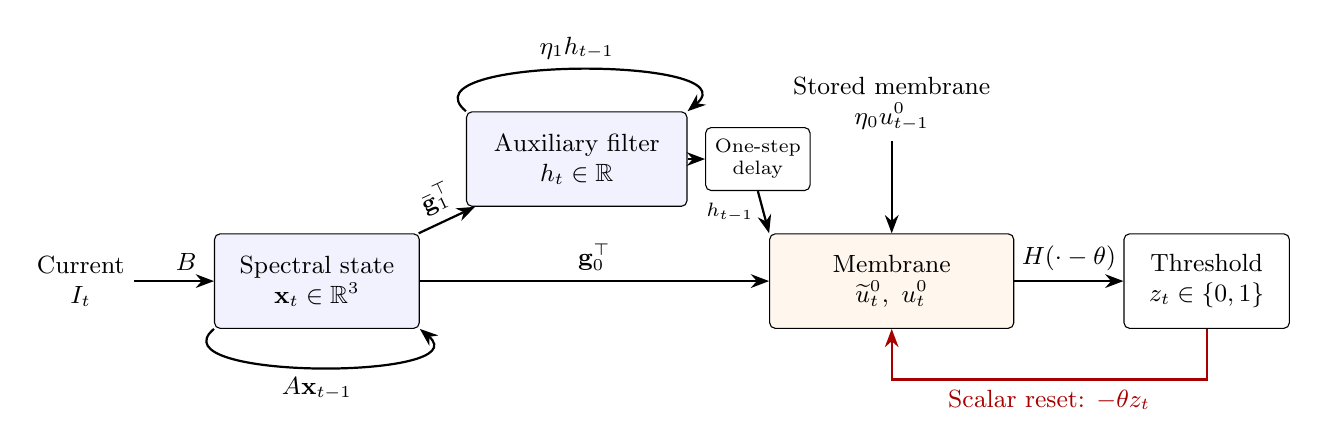
\begin{tikzpicture}[
  >=Stealth, font=\small,
  block/.style={draw,rounded corners=2pt,align=center,minimum height=12mm},
  mem/.style={block,fill=blue!5},
  arr/.style={->,thick}
]
\node[align=center] (in) at (0,0) {Current\\$I_t$};
\node[mem,minimum width=26mm] (x) at (3,0) {Spectral state\\$\mathbf x_t\in\R^3$};
\node[mem,minimum width=28mm] (h) at (6.3,1.55) {Auxiliary filter\\$h_t\in\R$};
\node[block,font=\scriptsize,minimum height=8mm,minimum width=13mm] (delay) at (8.6,1.55) {One-step\\delay};
\node[block,fill=orange!7,minimum width=31mm] (u) at (10.3,0)
  {Membrane\\$\widetilde u_t^0,\ u_t^0$};
\node[block,minimum width=21mm] (z) at (14.3,0) {Threshold\\$z_t\in\{0,1\}$};
\node[align=center] (prev) at (10.3,2.25) {Stored membrane\\$\eta_0u_{t-1}^0$};
\draw[arr] (in) -- node[above,pos=0.65] {$B$} (x);
\draw[arr] (x) -- node[above,sloped] {$\bar{\mathbf g}_1^\top$} (h);
\draw[arr] (x) -- node[above] {$\mathbf g_0^\top$} (u);
\draw[arr] (h.east) -- (delay.west);
\draw[arr] (delay.south) -- node[left,font=\scriptsize] {$h_{t-1}$} (u.north west);
\draw[arr] (prev.south) -- (u.north);
\draw[arr] (u) -- node[above] {$H(\cdot-\theta)$} (z);
\draw[arr,red!65!black] (z.south) -- (14.3,-1.25) -- node[below]
  {Scalar reset: $-\theta z_t$} (10.3,-1.25) -- (u.south);
\draw[arr] (x.south west) to[out=-140,in=-40] node[below] {$A\mathbf x_{t-1}$} (x.south east);
\draw[arr] (h.north west) to[out=140,in=40] node[above] {$\eta_1h_{t-1}$} (h.north east);
\end{tikzpicture}
\caption{SPRiF state organization. The spectral and auxiliary recurrences carry four memory and filter values. The membrane candidate combines the current spectral readout, the previous auxiliary value, and the previous post-reset membrane. The current reset acts on the scalar membrane. This diagram specifies equations rather than measured trajectories.}
\label{fig:organization}
\end{figure*}

\subsection{Absorbed Auxiliary Scaling}
\label{sec:scaling}

The coefficient of $h_{t-1}$ in Eq.~\eqref{eq:sprif} is fixed at one because its amplitude is already represented by the second readout row. To show this, consider the former scalar-reset parameterization with auxiliary coordinate $u_t^1$:
\begin{equation}
\begin{aligned}
u_t^1&=\eta_1u_{t-1}^1+\mathbf g_1^\top\mathbf x_t,\\
\widetilde u_t^0&=\eta_0u_{t-1}^0+\kappa u_{t-1}^1
                         +\mathbf g_0^\top\mathbf x_t.
\end{aligned}
\label{eq:legacy_scalar}
\end{equation}
In this conversion only, $\kappa$ denotes a time-independent legacy coupling. Define
\begin{equation}
h_t=\kappa u_t^1,\qquad
\bar{\mathbf g}_1=\kappa\mathbf g_1,\qquad
h_{-1}=\kappa u_{-1}^1.
\label{eq:absorption}
\end{equation}
Multiplication of the first recurrence by $\kappa$ and substitution into the second gives Eq.~\eqref{eq:sprif}. No division is required: at $\kappa=0$, $h_{-1}=0$ and $\bar{\mathbf g}_1=\mathbf0$ preserve the membrane and spike sequence. With corresponding initial states, the equality extends through a recurrent network because identical previous spikes give identical next currents.

This conversion assumes a free readout row and no separately required auxiliary output or amplitude constraint. SPRiF directly learns $\bar{\mathbf g}_1$; $\kappa$ is not a parameter of its current forward model. The auxiliary state remains present. Absorbing a coupling preserves fixed-parameter forward outputs for the scalar-reset formulation, while directly optimizing the product changes the optimization coordinates. Separate legacy penalties or constraints require an explicit new treatment. Historical training results therefore retain the model identities stated in Section~\ref{sec:provenance}.

\subsection{Spectral Basis, Controllability, and Effective Kernels}
\label{sec:kernels}

The poles of the spectral transition are
\begin{equation}
\spec(A)=\{\alpha,\rho e^{\mathrm i\omega},
                       \rho e^{-\mathrm i\omega}\}.
\label{eq:poles}
\end{equation}
For a unit impulse $I_0=1$, zero state at $t=-1$, and zero later current,
\begin{equation}
A^kB=
\begin{bmatrix}
(1-\alpha)\alpha^k\\
(1-\rho)\rho^k\cos(k\omega)\\
(1-\rho)\rho^k\sin(k\omega)
\end{bmatrix},\qquad k\geq0.
\label{eq:impulse}
\end{equation}
The first component gives monotone exponential retention. The other two provide phase-shifted responses with a common damping factor and frequency. Across neurons, learned decays, frequencies, and projections can distribute these responses over different temporal scales.

\begin{proposition}[Driven spectral coordinates]
For $\alpha,\rho\in(0,1)$ and $\omega\in(0,\pi)$, the pair $(A,B)$ in Eq.~\eqref{eq:AB} is controllable.
\label{prop:controllability}
\end{proposition}
\begin{IEEEproof}
Let $\mathcal C=[B,AB,A^2B]$. Expanding its determinant gives
\begin{equation}
\begin{aligned}
\det\mathcal C={}&(1-\alpha)(1-\rho)^2\rho\sin\omega\\
&{}\times(\alpha^2-2\alpha\rho\cos\omega+\rho^2).
\end{aligned}
\label{eq:controllability}
\end{equation}
Every factor is positive, since the last factor equals
$|\alpha-\rho e^{\mathrm i\omega}|^2$. Thus $\mathcal C$ has rank three.
\end{IEEEproof}

The proposition concerns the spectral block. Nearly zero $\sin\omega$ or small input factors can still produce poor numerical conditioning. It also does not imply that every mode is visible in a learned output: a readout can suppress a mode. Numerical singular values and readout scales are therefore relevant diagnostics.

Under the same impulse, the auxiliary response is
\begin{equation}
h_k=\sum_{\ell=0}^{k}\eta_1^{k-\ell}
                \bar{\mathbf g}_1^\top A^\ell B.
\label{eq:h_kernel}
\end{equation}
Write the membrane drive as
\begin{equation}
d_t=\mathbf g_0^\top\mathbf x_t+h_{t-1}.
\label{eq:drive}
\end{equation}
Its impulse kernel is
\begin{equation}
\begin{aligned}
k_d[k]={}&\mathbf g_0^\top A^kB\\
&{}+\sum_{\ell=0}^{k-1}\eta_1^{k-1-\ell}
                       \bar{\mathbf g}_1^\top A^\ell B ,
\end{aligned}
\label{eq:drive_kernel}
\end{equation}
where the sum is zero at $k=0$. The direct path responds immediately, whereas the auxiliary path first contributes at $k=1$. If $\xi$ denotes a formal unit-delay variable, the same transfer function is
\begin{equation}
\mathcal K_d(\xi)=
\left(\mathbf g_0^\top+
\frac{\xi}{1-\eta_1\xi}\bar{\mathbf g}_1^\top\right)
(I_3-\xi A)^{-1}B.
\label{eq:transfer}
\end{equation}
For a membrane with its spike reset suppressed, an additional factor $(1-\eta_0\xi)^{-1}$ gives its linear response. The actual stored membrane instead satisfies the exact expansion
\begin{equation}
\begin{aligned}
u_t^0={}&\eta_0^{t+1}u_{-1}^0
+\sum_{j=0}^{t}\eta_0^{t-j}d_j\\
&{}-\theta\sum_{j=0}^{t}\eta_0^{t-j}z_j .
\end{aligned}
\label{eq:membrane_unrolled}
\end{equation}
Thus Eq.~\eqref{eq:transfer} describes the linear drive, while the spike history remains in the membrane recurrence.

When an oscillatory pole has nonzero residue in the output kernel, a finite sum of modes with real positive poles cannot reproduce that kernel for all lags: equal rational transfer functions must have the same uncancelled poles. This specifies a distinction between the selected kernel families, not a universal advantage on a finite task. The real-mode control in Section~\ref{sec:controls} tests its empirical relevance with the same local capacity.

\subsection{Conditional State Bounds}
\label{sec:stability}

For fixed parameters and a specified current sequence, define
$\mathbf m_t=[\mathbf x_t^\top,h_t]^\top$. The memory pathway is
\begin{equation}
\mathbf m_t=F\mathbf m_{t-1}+LI_t,
\label{eq:memory_system}
\end{equation}
with
\begin{equation}
F=
\begin{bmatrix}
A&\mathbf0\\
\bar{\mathbf g}_1^\top A&\eta_1
\end{bmatrix},
\qquad
L=
\begin{bmatrix}B\\\bar{\mathbf g}_1^\top B\end{bmatrix}.
\label{eq:memory_matrices}
\end{equation}
The block-triangular structure gives
\begin{equation}
\spec(F)=\{\alpha,\rho e^{\mathrm i\omega},
               \rho e^{-\mathrm i\omega},\eta_1\}.
\label{eq:F_poles}
\end{equation}
All poles lie strictly inside the unit disk. This spectral property does not require $\|F\|_2<1$: its learned readout can produce transient amplification.

\begin{proposition}[Bounded local states]
Assume fixed finite readouts, finite initial states, $\theta>0$, the ranges in Eq.~\eqref{eq:constraints}, and $|I_t|\leq M$ for all $t\geq0$. Then $\mathbf x_t$, $h_t$, and $u_t^0$ in Eq.~\eqref{eq:sprif} remain bounded.
\label{prop:boundedness}
\end{proposition}
\begin{IEEEproof}
Let $q=\max(\alpha,\rho)<1$. Since the rotational block is $\rho R_\omega$, $\|A^k\|_2=q^k$. Unrolling the spectral recurrence gives
\begin{equation}
\|\mathbf x_t\|_2\leq
q^{t+1}\|\mathbf x_{-1}\|_2+
\|B\|_2M\frac{1-q^{t+1}}{1-q}.
\label{eq:x_bound}
\end{equation}
One uniform bound is
$X=\|\mathbf x_{-1}\|_2+\|B\|_2M/(1-q)$.
The auxiliary recurrence then yields
\begin{equation}
|h_t|\leq
\eta_1^{t+1}|h_{-1}|+
\|\bar{\mathbf g}_1\|_2X
       \frac{1-\eta_1^{t+1}}{1-\eta_1}.
\label{eq:h_bound}
\end{equation}
Put $H_*=|h_{-1}|+\|\bar{\mathbf g}_1\|_2X/(1-\eta_1)$ and
$D_*=\|\mathbf g_0\|_2X+H_*$. Then $|d_t|\leq D_*$.
Using $z_t\in\{0,1\}$ in Eq.~\eqref{eq:membrane_unrolled},
\begin{equation}
|u_t^0|\leq
\eta_0^{t+1}|u_{-1}^0|+
(D_*+\theta)\frac{1-\eta_0^{t+1}}{1-\eta_0},
\label{eq:u_bound}
\end{equation}
which is finite.
\end{IEEEproof}

The bounds describe the local forward states conditional on bounded current. They neither establish a contraction of the nonlinear recurrent network nor guarantee well-conditioned BPTT gradients. Large readouts and decays near one can yield large finite bounds. Coincident poles preserve boundedness but can change transients. Initialization, learned state scales, and recurrent responses are therefore evaluated alongside accuracy.

\subsection{Reset Identity and Recurrent Feedback}
\label{sec:reset}

Use superscripts $-$ and $+$ for values immediately before and after the current local reset. Equation~\eqref{eq:sprif} gives
\begin{equation}
\mathbf x_t^+=\mathbf x_t^-,
\qquad h_t^+=h_t^-,
\qquad u_t^{0,+}=\widetilde u_t^0-\theta z_t.
\label{eq:reset_identity}
\end{equation}
The reset increments of all four memory and filter coordinates are exactly zero for either spike outcome. This is an algebraic property of the current update, rather than an empirical robustness claim.

At fixed $I_t$, the memory-to-memory Jacobian is $F$ and contains no local threshold derivative. Its $k$-step intrinsic propagation is $F^k$. In a recurrent layer, however, changing a spike changes a later current by
\begin{equation}
\delta\mathbf I_{t+1}
       =W_{\rm rec}\,\delta\mathbf z_t
\label{eq:recurrent_feedback}
\end{equation}
when the external layer input is held fixed at that step. Later memory states can consequently differ. SI-DMS measures the complete response to membrane overwrite, forced firing, native reset, and recurrent propagation. The local identity specifies which immediate reset path is excluded; it does not isolate every cause of a later accuracy difference.

Single-threshold subtraction also leaves any excess voltage above one threshold in the stored membrane. Binary output is limited to one event per timestep, so a very large positive candidate need not become subthreshold after reset. This convention is part of Eq.~\eqref{eq:sprif} and differs from a threshold-quantized or multilevel discharge.

\subsection{Learning and Computational Accounting}
\label{sec:learning}

The hard threshold is used in the forward pass. For BPTT, its derivative is replaced by the multi-Gaussian surrogate used in the original specification~\cite{asrnn}:
\begin{equation}
\begin{aligned}
\psi(v)=\gamma\big[&
a_0\mathcal N(v-\theta;0,\sigma_0^2)\\
&-a_1\mathcal N(v-\theta;\mu_1,\sigma_1^2)\\
&-a_1\mathcal N(v-\theta;-\mu_1,\sigma_1^2)\big],
\end{aligned}
\label{eq:surrogate}
\end{equation}
where $\mathcal N(\cdot;\mu,\sigma^2)$ is the normalized Gaussian density,
$\sigma_0=0.5$, $\mu_1=0.5$, $\sigma_1=3.0$,
$a_0=1.15$, $a_1=0.15$, and $\gamma=0.5$.
The exact gradient treatment of reset and truncation is a protocol field in Section~\ref{sec:training}.

Each neuron stores $(x^0,x^1,x^2,h,u^0)$, for five state values. It learns the five raw variables associated with $\alpha,\rho,\omega,\eta_0,\eta_1$ and six entries of $\bar G$, for eleven dynamics coefficients. The count is not a claim of a globally minimal realization. Thresholds are fixed, and synaptic weights, biases, and output parameters are separate.

For a recurrent layer with input width $m$ and hidden width $n$, a dense input matrix, dense recurrent matrix, and one current bias per neuron contribute
\begin{equation}
N_{\rm layer}=mn+n^2+n+11n.
\label{eq:parameters}
\end{equation}
Output and additional architectural parameters are added according to their actual configuration. The persistent local state contains $5n$ scalar values, or $5nb_{\rm val}$ bytes when each value uses $b_{\rm val}$ bytes. This excludes weights, optimizer buffers, and BPTT activations. Local updates cost $O(n)$ per step; dense synaptic products cost $O(mn+n^2)$. Timing and peak memory require measurements under specified execution conditions.

\section{Experimental Setup}
\label{sec:setup}

\subsection{Tasks, Encodings, and Data Partitions}
\label{sec:data}

The five existing benchmarks span serialized images, physiological signals, dense speech features, and event-based speech. Their roles differ: S-MNIST tests long sequential integration; PS-MNIST disrupts local pixel order; QTDB uses a label at each timestep; GSC classifies a complete feature sequence; and SHD uses sparse cochlear events. Dataset sources define the original data, while the encodings below follow the supplied experimental specification.

S-MNIST and PS-MNIST use MNIST~\cite{lecun1998gradient} images as 784 scalar pixel inputs. PS-MNIST uses a permutation generated from the run seed and held fixed within that run. Every compared model at the same seed uses the same permutation. Variation across seeds therefore includes permutation variation as well as the training realization. The pixel normalization and the training/validation partition for the new runs remain \pending.

QTDB uses the QT Database~\cite{laguna1997database} with the event encoding adopted in ASRNN~\cite{asrnn}. Two normalized ECG channels are smoothed and converted into positive and negative first-difference events, yielding four input streams. Six waveform classes are predicted at each labeled timestep. The split must identify the original records or subjects from which windows are derived, so that overlapping or related windows are assigned consistently. Record identifiers, window lengths and overlaps, normalization sources, event thresholds, and the timestep interpretation are \pending. These fields are necessary to interpret a new QTDB accuracy.

GSC uses one-second utterances from Speech Commands~\cite{warden2018speech}. The supplied configuration uses 40 mel bins with first- and second-order deltas, producing 120 input features across 101 frames and a 12-class output. Hidden spikes are pooled over time before classification. The dataset release, exact class mapping including any silence or unknown classes, partition counts, audio normalization, and feature extraction constants are \pending.

SHD uses the 700-channel cochlear spike trains of Spiking Heidelberg Digits~\cite{cramer2022heidelberg}, with 20 classes. The supplied configuration accumulates output evidence after a warm-up period. Bin duration, temporal truncation or padding, the warm-up length, output recurrence, validation partition, and handling of variable sequence length are \pending.

The new runs use a fixed training/validation/test partition. Where no validation partition is specified, it will be selected from training data before formal training. Validation chooses the checkpoint using a predetermined metric, with the earliest checkpoint resolving a tie; the test set is used for final evaluation. The actual split identifiers, sample counts, validation frequency, and task-specific selection metric remain \pending. These new selection rules are not inferred retrospectively for the historical runs.

\subsection{Networks, Optimization, and Initialization}
\label{sec:training}

Table~\ref{tab:configuration} collects the original manuscript's task-specific settings as candidate starting configurations. The table distinguishes an available configuration from a completed run of Eq.~\eqref{eq:sprif}. In the new networks, all spiking hidden neurons use the eleven-coefficient definition. The network widths and optimization settings will be frozen before formal evaluation; any subsequent change creates a new configuration and requires a new set of formal runs.

\begin{table*}[t]
\caption{Candidate benchmark settings from the original manuscript. These values provide the starting configuration; their retention and the pending fields in Section~\ref{sec:training} must be resolved before the new runs. Timescale intervals are in timesteps.}
\label{tab:configuration}
\centering
\small
\setlength{\tabcolsep}{5pt}
\begin{tabular}{@{}lccccc@{}}
\toprule
Item & S-MNIST & PS-MNIST & QTDB & GSC & SHD\\
\midrule
Input / output width & 1 / 10 & 1 / 10 & 4 / 6 & 120 / 12 & 700 / 20\\
Recurrent hidden widths & 64, 210 & 64, 210 & 31 & 300 & 64\\
Epochs & 150 & 150 & 250 & 150 & 100\\
Batch size & 512 & 512 & 128 & 128 & 100\\
Adam learning rate & $10^{-2}$ & $10^{-2}$ & $10^{-2}$ & $5\,10^{-3}$ & $10^{-2}$\\
StepLR factor / interval & 0.1 / 50 & 0.1 / 50 & 0.65 / 100 & 0.5 / 30 & 0.5 / 20\\
Fixed threshold $\theta$ & 1.0 & 1.0 & 0.6 & 0.8 & 1.0\\
$\tau_\alpha$ & $[2,60]$ & $[2,60]$ & $[20,120]$ & $[10,80]$ & $[10,80]$\\
$\tau_\rho$ & $[2,40]$ & $[2,40]$ & $[4,30]$ & $[4,30]$ & $[4,30]$\\
$\tau_{\eta_0},\tau_{\eta_1}$ & $[0.8,10]$ & $[0.8,10]$ & $[0.8,8]$ & $[0.8,8]$ & $[0.8,8]$\\
$\omega/\pi$ & $[0.04,0.50]$ & $[0.04,0.50]$ & $[0.02,0.20]$ & $[0.04,0.40]$ & $[0.04,0.40]$\\
\bottomrule
\end{tabular}
\end{table*}

All tasks use cross-entropy and the surrogate in Eq.~\eqref{eq:surrogate}. The supplied S-MNIST and PS-MNIST configuration uses truncated BPTT with chunks of 262 steps. GSC pools hidden spikes by a temporal mean; QTDB optimizes labeled timesteps; SHD accumulates readout evidence after warm-up. Exact logit formation for each task, loss weighting or masking, optimizer constants, gradient clipping, weight decay, and the gradient treatment of reset are \pending. For truncation, state carryover, graph detachment, and chunk aggregation must be specified separately: carrying a numerical state and carrying its computation graph are different operations.

For each decay $q\in\{\alpha,\rho,\eta_0,\eta_1\}$, a positive time constant $\tau_q$ maps to
\begin{equation}
q=\exp(-1/\tau_q),\qquad
q_{\rm raw}=\log\frac{q}{1-q}.
\label{eq:decay_init}
\end{equation}
Frequency initialization uses the analogous inverse sigmoid of $\omega/\pi$. The interval alone does not define the sampling distribution; the distribution and neuron-wise sampling rule are \pending.

The two rows of $\bar G$ are initialized and optimized directly. If a reproducible legacy scalar-reset draw is used, its second row is converted by Eq.~\eqref{eq:absorption}; the legacy coefficient is discarded after initialization. A direct draw for the new row is also possible. The selected rule, scale, and any regularization remain \pending. Controls share that rule and pair common initialization variables where meaningful. Finite-precision treatment of sigmoid endpoints and very small input-vector norms must also be fixed before evaluation.

Formal repetitions use seeds $\{0,1,2,42,1111\}$. Development runs and their configuration choices are recorded separately. Preliminary runs can enter the formal set only if the predeclared configuration is retained; runs used to alter it become development runs. Infrastructure failures can be retried at the same seed, whereas model numerical failures must be retained in the reported run status. Software versions, hardware, precision, reproducibility settings, and retry criteria for the new runs are \pending.

\subsection{Controls with Matched Local Capacity}
\label{sec:controls}

The structural comparison uses SPRiF, \mr, and \rmodes\ on PS-MNIST and SHD. All three store five state values and learn eleven dynamics coefficients per neuron. They use the same hidden widths, data partitions, readout, training budget, selection rule, and seed-paired input conditions. The comparison tests two specified state organizations, with their scale and conditioning diagnostics.

\subsubsection{\mr}
Compute the current spectral state $\mathbf x_t^-$, both readouts, the auxiliary state, and the membrane spike as in SPRiF. After firing, additionally update
\begin{equation}
\begin{aligned}
\widehat B&=\frac{B}{\|B\|_2},\qquad \gamma_{\rm mem}=1,\\
\mathbf x_t^+&=\mathbf x_t^--\gamma_{\rm mem}\theta z_t\widehat B.
\end{aligned}
\label{eq:memory_reset_control}
\end{equation}
The next step uses $\mathbf x_t^+$. The current $h_t$ was computed from $\mathbf x_t^-$ and receives no extra direct reset. The fixed coefficient adds no learned parameter.

This control introduces one reproducible soft-reset direction through spectral memory. It does not reset all four memory and filter values. Its effect depends on input, state, and readout scales, so the analysis records $\|\Delta\mathbf x_t\|_2$, $\|B\|_2$, both readout norms, and the induced drive change. The numerical safeguard for a tiny $\|B\|_2$ is \pending. A fixed reset magnitude alone does not establish equal functional perturbation strength across different coordinates.

\subsubsection{\rmodes}
Replace the spectral matrices by
\begin{equation}
A_{\rm real}=\diag(a_1,a_2,a_3),\qquad
B_{\rm real}=\begin{bmatrix}1-a_1\\1-a_2\\1-a_3\end{bmatrix},
\label{eq:real_control}
\end{equation}
where $a_i=\sigma(a_{i,\rm raw})$ are independently learned. Three real decay parameters replace $\alpha,\rho,\omega$. The auxiliary filter, membrane, scalar reset, and six readout entries are retained.

The first real-mode time constant uses the $\tau_\alpha$ interval, and the other two use independent draws from the $\tau_\rho$ interval. Distinct poles make the three coordinates controllable, whereas repeated or nearly repeated poles can reduce effective rank or conditioning. Singular values of $[B_{\rm real},A_{\rm real}B_{\rm real},A_{\rm real}^2B_{\rm real}]$, with a declared rank tolerance (\pending), are reported along with input and readout scales. This control tests real versus real-plus-rotational organization at matched capacity. Setting the original rotation to zero would leave its third coordinate undriven from zero initialization and would test a different, degenerate configuration.

\subsection{Controlled Baselines and a Full-Method Comparison}
\label{sec:baselines}

TC-LIF~\cite{tclif} and BRF~\cite{brf} are compared on PS-MNIST and SHD under the common input, partition, readout, validation, and seed protocol. Their native dynamics and initialization are retained and specified in the final configuration. Widths are chosen to bring total trainable parameters as close as practicable to SPRiF, targeting a difference within 5\%. Actual widths, parameter counts, native settings, and the achieved budget differences are \pending. Equal width is not treated as evidence of equal parameter budget.

DMP-SNN~\cite{sun2026dmp} is evaluated on PS-MNIST using its native layer-shared memory organization and full architecture. Compatible data and selection settings are shared; architectural, optimization, and budget differences are stated with the results. This comparison concerns a complete method rather than a neuron substitution. ASRNN~\cite{asrnn} is included in SI-DMS with the common recurrent task protocol. The current related-work comparison with PMSN and D-RF concerns equations and state organization; the empirical comparison set is the one specified here.

\subsection{SI-DMS: Task and Spike Intervention}
\label{sec:sidms}

SI-DMS is a generated match/non-match task with one recurrent hidden layer. Thirty input channels form three groups of ten: left cue, right cue, and background noise. Poisson spike trains encode the inputs. A 50-ms pre-period is followed by a 100-ms first cue, a variable delay, and a 100-ms second cue. The two cues define the binary target. Matching cues have the same identity but independent spike realizations. The hidden layer has 64 neurons and connects to a two-class nonspiking leaky readout. Table~\ref{tab:sidms_setup} gives the candidate training budget and the comparison grid.

\begin{table}[t]
\caption{SI-DMS protocol. Available task settings are retained from the supplied specification; unresolved generator and evaluation constants are identified in the text.}
\label{tab:sidms_setup}
\centering
\small
\begin{tabularx}{\columnwidth}{@{}>{\raggedright\arraybackslash}p{0.32\columnwidth}>{\raggedright\arraybackslash}X@{}}
\toprule
Item & Setting\\
\midrule
Architecture & $30$ inputs, $64$ recurrent hidden neurons, $2$ leaky outputs\\
Training delays & $200,400,800,1600$ ms\\
Evaluation delays & Training delays and $2500$ ms\\
Models & SPRiF, \mr, ASRNN\\
Clean training & No forced intervention\\
Intervention training & $K\in\{0,1,2,4,8\}$; nominal $f=15\%$\\
Primary stress & $K=40$, nominal $f=15\%$\\
Other evaluation counts & $K=0,1,2,4,8,16,32$\\
Candidate optimizer & Adam, learning rate $3\times10^{-3}$\\
Candidate budget & $3000$ updates, batch $256$, gradient clip $1.0$\\
Rate regularization & Natural-rate target $0.10$, weight $0.05$\\
Formal seeds & $0,1,2,42,1111$ per model and training condition\\
\bottomrule
\end{tabularx}
\end{table}

At each of $K$ selected delay timesteps, the designated units' membrane candidates are overwritten with a value $v_{\rm set}>\theta$ immediately before thresholding. Their actual spikes trigger native reset and enter the recurrent pathway. For SPRiF, $\mathbf x_t$ and $h_t$ have already been computed normally and are not overwritten. A forced event is distinguished from natural firing when computing rate regularization. The protocol consequently changes membrane voltage, spike generation, reset, and future feedback together.

Clean and intervention training use the same number of updates and generated task conditions. Each formal seed supplies matched evaluation inputs and external intervention schedules across models and across clean/stressed replays. The timestep, cue/noise rates, identity and label sampling law, validation and test sample counts, intervention time sampling law, selected-unit rounding rule, $v_{\rm set}$, output leak, loss window, and exclusion of forced events from the rate term are \pending. In the former task, nominal 15\% corresponded to 10 of 64 units; the exact rule for the new runs must be stated rather than inferred from the percentage alone.

For seed $s$, delay $d$, count $K$, and fraction $f$, the paired loss is
\begin{equation}
\Delta_{s,d}(K,f)=
\Acc_{s,d}(0)-\Acc_{s,d}(K,f).
\label{eq:paired_loss}
\end{equation}
Accuracies are percentages, so $\Delta$ is measured in percentage points. Each seed is averaged over the five evaluation delays before calculating the across-seed summary. The 2500-ms delay is also reported separately because it lies outside the training set. Counts above eight are outside the intervention-training range. Clean capability, stressed capability, and their paired loss are all required to interpret memory preservation.

\subsection{Initialization, State Diagnostics, and Cost Measurement}
\label{sec:diagnostics}

Initialization sensitivity uses PS-MNIST with all time-constant intervals multiplied by $0.5$, $1$, or $2$, while holding the frequency interval, readout rule, optimizer, and other settings fixed. The five standard-initialization runs are reused, and the other two ranges each use five formal seeds. The decay transform remains Eq.~\eqref{eq:decay_init}.

The analysis records initialized and learned decays and frequencies, state magnitudes, readout norms, natural firing rates, and numerical failures. A specified tolerance (\pending) defines proximity to a parameter boundary. Impulse diagnostics inject a unit current into the fixed-parameter local memory pathway and compare the resulting $\mathbf x_t$, $h_t$, and drive with Eqs.~\eqref{eq:impulse}--\eqref{eq:drive_kernel}. Checkpoint selection, the displayed-neuron rule, and the observation horizon are \pending. Immediate pre/post-reset trajectories test Eq.~\eqref{eq:reset_identity}; recurrent clean/stressed replay is treated as a separate network diagnostic.

Cost reporting covers SPRiF, TC-LIF, and BRF on PS-MNIST and SHD. It includes total trainable parameters, dynamics coefficients, persistent state bytes, inference latency, peak device memory, and training time for the stated budget. Timing uses both batch one and the task training batch, with matched device, precision, input length, and software settings. The candidate timing protocol uses 20 warm-up calls and 100 timed repetitions with device synchronization, reporting median and interquartile range. Exact runtime settings and hardware are \pending. Full-method DMP-SNN costs are identified with its own configuration. GPU latency and operation counts are not measurements of neuromorphic-device energy.

\subsection{Metrics and Statistical Units}
\label{sec:statistics}

Sequence accuracy is the primary metric for S-MNIST, PS-MNIST, GSC, SHD, and SI-DMS. QTDB accuracy uses correctly classified labeled timesteps divided by all evaluated labeled timesteps; masking rules are \pending. Per-class precision, recall, and macro-F1 are included for QTDB to clarify whether overall accuracy reflects class imbalance; the class mapping and aggregation rule remain \pending.

For $S=5$ independent training seeds with scores $a_s$, report
\begin{equation}
\bar a=\frac1S\sum_{s=1}^{S}a_s,\qquad
s_a=\sqrt{\frac1{S-1}\sum_{s=1}^{S}(a_s-\bar a)^2}.
\label{eq:statistics}
\end{equation}
Structural comparisons also report every seed-paired difference and its mean and sample standard deviation. Test examples, delay conditions, and repeated timings are not independent training repetitions. With five seeds, a small difference can remain uncertain; a superiority statement requires evidence beyond a positive point estimate. Published comparator numbers, if included later, will be identified by their original protocol and kept separate from the controlled reruns.

\section{Results and Discussion}
\label{sec:results}

\subsection{Evidence Status and Historical Provenance}
\label{sec:provenance}

No new training measurements are available for the eleven-coefficient neuron in Eq.~\eqref{eq:sprif}. In this manuscript, \pending\ denotes an unavailable result or protocol value. The analytic conclusions in Section~\ref{sec:model} follow from the equations; performance and cost conclusions require the measurements organized below.

The historical Full model stored five values and learned thirteen dynamics coefficients, including a separate auxiliary coupling and a nonmembrane reset coefficient. Its scalar-reset variant retained the independent coupling and learned twelve coefficients. Table~\ref{tab:historical} preserves their reported five-seed benchmark accuracies. The Full-to-scalar change alters the model; the subsequent scaling absorption in Section~\ref{sec:scaling} is a fixed-parameter conversion of the scalar-reset variant. Neither step supplies the outcomes of new training.

\begin{table}[t]
\caption{Historical benchmark accuracies (\%) from the original manuscript. Columns retain their original model identities and reported five-seed summaries. A dash denotes an unreported entry.}
\label{tab:historical}
\centering
\small
\begin{tabular}{@{}lcc@{}}
\toprule
Task & Former Full (13) & Former scalar (12)\\
\midrule
S-MNIST & $99.28\pm0.06$ & ---\\
PS-MNIST & $95.86\pm0.14$ & $95.32\pm0.18$\\
QTDB & $88.43\pm0.36$ & $87.78\pm0.30$\\
GSC & $94.55\pm0.31$ & $94.22\pm0.22$\\
SHD & $91.52\pm0.46$ & ---\\
\bottomrule
\end{tabular}
\end{table}

Historical SI-DMS also used a different protocol: three seeds and intervention training. At nominal $f=15\%$, the original Full model reported clean accuracy $100.0\pm0.0\%$ and loss $0.2\pm0.2$ percentage points at $K=40$; the former scalar-reset variant reported $99.4\pm0.0\%$ and loss $4.2\pm0.2$ points. These summaries do not populate Table~\ref{tab:sidms_results}. The original learned-reset, loss-landscape, impulse, and perturbation plots likewise belong to the historical checkpoints. The current manuscript uses an equation-based schematic and reserves empirical diagnostics for the new models.

\subsection{Five-Benchmark Performance}
\label{sec:main_results}

Table~\ref{tab:main_results} reports the new parameterization at the complete-network level. Total parameters must include all synaptic, bias, dynamics, and output parameters. The five-seed summaries will use the frozen data and checkpoint protocol. Comparison of new and historical accuracy must account for any change in partition, preprocessing, selection, or initialization; such a difference cannot automatically be attributed to removing a reset coefficient.

\begin{table}[t]
\caption{SPRiF with five states and eleven learned dynamics coefficients per neuron. Entries require new measurements; accuracy uses five seeds.}
\label{tab:main_results}
\centering
\small
\begin{tabular}{@{}lcc@{}}
\toprule
Task & Accuracy (\%) & Total parameters\\
\midrule
S-MNIST & \pending & \pending\\
PS-MNIST & \pending & \pending\\
QTDB & \pending & \pending\\
GSC & \pending & \pending\\
SHD & \pending & \pending\\
\bottomrule
\end{tabular}
\end{table}

The empirical interpretation for the five tasks is \pending. For QTDB, per-class and macro-F1 results are also \pending. These results will determine whether performance is consistent across temporal modalities or concentrated in a particular task regime.

\subsection{Structural Controls and Related Baselines}
\label{sec:structural_results}

Table~\ref{tab:controlled_results} organizes the matched-capacity controls and the controlled neuron baselines. The two structural contrasts are SPRiF minus \mr\ and SPRiF minus \rmodes. Every seed-paired accuracy difference is included in Table~\ref{tab:paired_results}; their means and sample standard deviations are \pending. TC-LIF and BRF comparisons require the actual total-parameter matches, while DMP-SNN retains its native architecture.

\begin{table*}[t]
\caption{New controlled comparisons and the PS-MNIST full-method comparison. The first three models have five states and eleven local coefficients at the same width. TC-LIF and BRF target matched total parameter budgets; DMP-SNN uses its native architecture. A dash denotes a task outside the comparison scope.}
\label{tab:controlled_results}
\centering
\small
\begin{tabular}{@{}lcccc@{}}
\toprule
Model & PS-MNIST (\%) & SHD (\%) & PS-MNIST parameters & SHD parameters\\
\midrule
SPRiF & \pending & \pending & \pending & \pending\\
\mr & \pending & \pending & \pending & \pending\\
\rmodes & \pending & \pending & \pending & \pending\\
\midrule
TC-LIF & \pending & \pending & \pending & \pending\\
BRF & \pending & \pending & \pending & \pending\\
\midrule
DMP-SNN (native) & \pending & --- & \pending & ---\\
\bottomrule
\end{tabular}
\end{table*}

\begin{table*}[t]
\caption{Seed-paired SPRiF accuracy gains over the two matched-capacity controls, in percentage points. All formal seeds are shown. The paired data and numerical conditioning diagnostics are required for interpretation.}
\label{tab:paired_results}
\centering
\small
\begin{tabular}{@{}lcccc@{}}
\toprule
& \multicolumn{2}{c}{PS-MNIST} & \multicolumn{2}{c}{SHD}\\
\cmidrule(lr){2-3}\cmidrule(lr){4-5}
Seed & vs.\ \mr & vs.\ \rmodes & vs.\ \mr & vs.\ \rmodes\\
\midrule
0 & \pending & \pending & \pending & \pending\\
1 & \pending & \pending & \pending & \pending\\
2 & \pending & \pending & \pending & \pending\\
42 & \pending & \pending & \pending & \pending\\
1111 & \pending & \pending & \pending & \pending\\
\bottomrule
\end{tabular}
\end{table*}

A difference against \mr\ would characterize the tested input-direction spectral reset at its recorded scale. A difference against \rmodes\ would characterize the selected real versus rotational memory organization. These controls address a state-and-coefficient-capacity explanation, while their conditioning and scale measurements address additional confounds. The relevant interpretation remains \pending; neither the parameter count nor the kernel derivation establishes task superiority.

\subsection{Spike Intervention and Delay Generalization}
\label{sec:sidms_results}

Table~\ref{tab:sidms_results} reports the primary $K=40$, nominal $f=15\%$ condition under clean and intervention training. The across-delay summary and the 2500-ms result are shown together. Curves across intervention count and the pre/post-reset state trajectories are \pending.

\begin{table*}[t]
\caption{SI-DMS at $K=40$ and nominal $f=15\%$. Accuracies are percentages and paired losses are percentage points. Each delay-averaged value is formed within a seed, then summarized over five independent training seeds. The unseen 2500-ms delay is reported separately.}
\label{tab:sidms_results}
\centering
\small
\setlength{\tabcolsep}{5pt}
\begin{tabular}{@{}llcccccc@{}}
\toprule
& & \multicolumn{3}{c}{Five-delay mean} & \multicolumn{3}{c}{2500-ms delay}\\
\cmidrule(lr){3-5}\cmidrule(lr){6-8}
Training & Model & Clean & Stress & $\Delta_{40}$ & Clean & Stress & $\Delta_{40}$\\
\midrule
Clean & SPRiF & \pending & \pending & \pending & \pending & \pending & \pending\\
Clean & \mr & \pending & \pending & \pending & \pending & \pending & \pending\\
Clean & ASRNN & \pending & \pending & \pending & \pending & \pending & \pending\\
\midrule
Intervention & SPRiF & \pending & \pending & \pending & \pending & \pending & \pending\\
Intervention & \mr & \pending & \pending & \pending & \pending & \pending & \pending\\
Intervention & ASRNN & \pending & \pending & \pending & \pending & \pending & \pending\\
\bottomrule
\end{tabular}
\end{table*}

Clean accuracy establishes whether each model can retain the cue before stress. The paired loss measures degradation relative to that capability, and stressed accuracy prevents a low loss at poor clean performance from being interpreted as useful protection. A benefit present under clean training would support a broader interpretation than a benefit restricted to intervention training. Since the intervention changes several connected paths, the result concerns complete model response; attributing all of a difference to an isolated reset path would require an additional path-isolation analysis.

\subsection{Resource Cost and Learned Dynamics}
\label{sec:cost_results}

Table~\ref{tab:cost_results} places the measured neuron comparisons under common execution conditions. Persistent state is counted from the actual layer widths and scalar precision. Latencies are per complete sequence; peak memory and training time are associated with the stated batch and training budget. The table separates storage predicted by the state definition from the measured costs of executing and training the network. DMP-SNN full-method cost and its configuration differences remain \pending.

\begin{table*}[t]
\caption{Resource measurements for the controlled neuron comparisons. State storage excludes parameters and BPTT activations. Latency summaries require synchronized timings under the same device and precision. $B_{\rm train}$ is the task training batch.}
\label{tab:cost_results}
\centering
\small
\setlength{\tabcolsep}{4pt}
\begin{tabular}{@{}llcccccc@{}}
\toprule
Task & Model & Parameters & State (KiB) & \multicolumn{2}{c}{Latency (ms)} & Peak (MiB) & Train (h)\\
\cmidrule(lr){5-6}
& & & & Batch 1 & $B_{\rm train}$ & &\\
\midrule
PS-MNIST & SPRiF & \pending & \pending & \pending & \pending & \pending & \pending\\
PS-MNIST & TC-LIF & \pending & \pending & \pending & \pending & \pending & \pending\\
PS-MNIST & BRF & \pending & \pending & \pending & \pending & \pending & \pending\\
\midrule
SHD & SPRiF & \pending & \pending & \pending & \pending & \pending & \pending\\
SHD & TC-LIF & \pending & \pending & \pending & \pending & \pending & \pending\\
SHD & BRF & \pending & \pending & \pending & \pending & \pending & \pending\\
\bottomrule
\end{tabular}
\end{table*}

Accuracy and cost must be interpreted together. Additional states require storage even when local updates are linear in width, and dense recurrence can dominate computation. The current theoretical specification supplies neither a latency speedup nor a hardware-energy claim.

The initialization comparison in Table~\ref{tab:initialization_results} tests whether a useful operating range extends beyond the original intervals. Boundary fractions, state magnitudes, firing rates, spectral conditioning, and learned drive kernels are \pending. The local algebra predicts the kernel for any fixed parameters; observed training behavior must establish which parameter regimes are actually reached.

\begin{table}[t]
\caption{PS-MNIST initialization sensitivity. All time-constant intervals are scaled together, with frequency and other settings fixed. The standard-range result reuses the main runs.}
\label{tab:initialization_results}
\centering
\small
\begin{tabular}{@{}lccc@{}}
\toprule
Interval scale & Accuracy (\%) & Natural rate & Failed runs\\
\midrule
$0.5$ & \pending & \pending & \pending\\
$1$ & \pending & \pending & \pending\\
$2$ & \pending & \pending & \pending\\
\bottomrule
\end{tabular}
\end{table}

\subsection{Scope and Limitations}
\label{sec:limitations}

SPRiF restricts intrinsic memory to three spectral coordinates and an auxiliary filter. Learned readouts can cancel modes, and near-boundary parameters can impair conditioning within the proved stability range. The resulting family is a constrained temporal realization.

The immediate reset identity does not isolate recurrent feedback or the other changes made by SI-DMS. Interpretation of the controls depends on their reset direction, perturbation scale, conditioning, and initialization. Absorbed scaling preserves fixed-parameter outputs but can change optimization and regularization. Performance, robustness, and resource tradeoffs require the pending measurements.

\section{Conclusion}
\label{sec:conclusion}

SPRiF couples a real-plus-rotational spectral block and an auxiliary linear filter to a scalar membrane with subtractive reset. The five-state parameterization learns eleven local dynamics coefficients and retains a one-step auxiliary drive. Its equations establish a controllable spectral basis, an explicit effective drive kernel, bounded local states under bounded current, and zero immediate reset increments in all four memory and filter coordinates. The empirical protocol connects these properties to matched-capacity controls, temporal benchmarks, recurrent intervention, and measured resource costs. New measurements are required to determine the practical value of this organization.

% Generated by IEEEtran.bst, version: 1.14 (2015/08/26)
\begin{thebibliography}{10}
\providecommand{\url}[1]{#1}
\csname url@samestyle\endcsname
\providecommand{\newblock}{\relax}
\providecommand{\bibinfo}[2]{#2}
\providecommand{\BIBentrySTDinterwordspacing}{\spaceskip=0pt\relax}
\providecommand{\BIBentryALTinterwordstretchfactor}{4}
\providecommand{\BIBentryALTinterwordspacing}{\spaceskip=\fontdimen2\font plus
\BIBentryALTinterwordstretchfactor\fontdimen3\font minus
  \fontdimen4\font\relax}
\providecommand{\BIBforeignlanguage}[2]{{%
\expandafter\ifx\csname l@#1\endcsname\relax
\typeout{** WARNING: IEEEtran.bst: No hyphenation pattern has been}%
\typeout{** loaded for the language `#1'. Using the pattern for}%
\typeout{** the default language instead.}%
\else
\language=\csname l@#1\endcsname
\fi
#2}}
\providecommand{\BIBdecl}{\relax}
\BIBdecl

\bibitem{asrnn}
B.~Yin, F.~Corradi, and S.~M. Boht{\'{e}}, ``Accurate and efficient time-domain
  classification with adaptive spiking recurrent neural networks,''
  \emph{Nature Machine Intelligence}, vol.~3, pp. 905--913, 2021.

\bibitem{adlif}
M.~Baronig, R.~Ferrand, S.~Sabathiel, and R.~Legenstein, ``Advancing
  spatio-temporal processing through adaptation in spiking neural networks,''
  \emph{Nature Communications}, vol.~16, p. 5776, 2025.

\bibitem{izhikevich_rf}
E.~M. Izhikevich, ``Resonate-and-fire neurons,'' \emph{Neural Networks},
  vol.~14, no. 6-7, pp. 883--894, 2001.

\bibitem{brf}
S.~Higuchi, S.~Kairat, S.~Bohte, and S.~Otte, ``Balanced resonate-and-fire
  neurons,'' in \emph{Proceedings of the 41st International Conference on
  Machine Learning}, ser. Proceedings of Machine Learning Research, vol.
  235.\hskip 1em plus 0.5em minus 0.4em\relax PMLR, 2024, pp. 18\,305--18\,323.

\bibitem{drf}
D.~Zhang, M.~Zhang, S.~Wang, J.~Wang, W.~Wei, Z.~Ma, G.~Wang, Y.~Yang, and
  H.~Li, ``Dendritic resonate-and-fire neuron for effective and efficient long
  sequence modeling,'' in \emph{Advances in Neural Information Processing
  Systems (NeurIPS)}, vol.~38, 2025.

\bibitem{tclif}
S.~Zhang, Q.~Yang, C.~Ma, J.~Wu, H.~Li, and K.~C. Tan, ``{TC-LIF}: A
  two-compartment spiking neuron model for long-term sequential modelling,'' in
  \emph{Proceedings of the AAAI Conference on Artificial Intelligence},
  vol.~38, 2024, pp. 16\,838--16\,847.

\bibitem{dhsnn}
H.~Zheng, Z.~Zheng, R.~Hu, B.~Xiao, Y.~Wu, F.~Yu, X.~Liu, G.~Li, and L.~Deng,
  ``Temporal dendritic heterogeneity incorporated with spiking neural networks
  for learning multi-timescale dynamics,'' \emph{Nature Communications},
  vol.~15, p. 277, 2024.

\bibitem{pmsn2026}
X.~Chen, J.~Wu, C.~Ma, Y.~Yan, H.~Liu, Y.~Wu, and K.~C. Tan, ``{PMSN}: A
  parallel multi-compartment spiking neuron for multiscale temporal
  processing,'' \emph{IEEE Transactions on Neural Networks and Learning
  Systems}, 2026, Early Access.

\bibitem{sun2026dmp}
P.~Sun, Z.~Su, J.~Achterberg, G.~Indiveri, D.~F.~M. Goodman, and D.~Akarca,
  ``Algorithm--hardware co-design of neuromorphic networks with dual memory
  pathways,'' \emph{Nature Machine Intelligence}, vol.~8, pp. 901--912, 2026.

\bibitem{spikingssms}
S.~Shen, C.~Wang, R.~Huang, Y.~Zhong, Q.~Guo, Z.~Lu, J.~Zhang, and L.~Leng,
  ``{SpikingSSMs}: Learning long sequences with sparse and parallel spiking
  state space models,'' in \emph{Proceedings of the AAAI Conference on
  Artificial Intelligence}, vol.~39, 2025, pp. 20\,380--20\,388.

\bibitem{nisnna2025}
C.~Zhang, W.~Pan, and C.~Della~Santina, ``{NiSNN-A}: Noniterative spiking
  neural network with attention with application to motor imagery {EEG}
  classification,'' \emph{IEEE Transactions on Neural Networks and Learning
  Systems}, vol.~36, no.~8, pp. 14\,298--14\,312, 2025.

\bibitem{imlspikeformer2026}
Z.~Song, S.~Zhang, Y.~Chou, J.~Wu, and H.~Li, ``{IML-Spikeformer}: Input-aware
  multilevel spiking transformer for speech processing,'' \emph{IEEE
  Transactions on Neural Networks and Learning Systems}, vol.~37, no.~3, pp.
  1377--1389, 2026.

\bibitem{stdl2026}
C.~Ma, X.~Chen, K.~C. Tan, and J.~Wu, ``Spatiotemporal decoupled learning for
  spiking neural networks,'' \emph{IEEE Transactions on Neural Networks and
  Learning Systems}, vol.~37, no.~9, pp. 4597--4611, 2026.

\bibitem{lecun1998gradient}
\BIBentryALTinterwordspacing
Y.~LeCun, L.~Bottou, Y.~Bengio, and P.~Haffner, ``Gradient-based learning
  applied to document recognition,'' \emph{Proceedings of the IEEE}, vol.~86,
  no.~11, pp. 2278--2324, 1998. [Online]. Available:
  \url{https://doi.org/10.1109/5.726791}
\BIBentrySTDinterwordspacing

\bibitem{laguna1997database}
\BIBentryALTinterwordspacing
P.~Laguna, R.~G. Mark, A.~L. Goldberger, and G.~B. Moody, ``A database for
  evaluation of algorithms for measurement of {QT} and other waveform intervals
  in the {ECG},'' in \emph{Computers in Cardiology}, vol.~24, 1997, pp.
  673--676. [Online]. Available:
  \url{https://physionet.org/content/qtdb/1.0.0/doc/}
\BIBentrySTDinterwordspacing

\bibitem{warden2018speech}
\BIBentryALTinterwordspacing
P.~Warden, ``Speech commands: A dataset for limited-vocabulary speech
  recognition,'' \emph{CoRR}, vol. abs/1804.03209, 2018. [Online]. Available:
  \url{https://arxiv.org/abs/1804.03209}
\BIBentrySTDinterwordspacing

\bibitem{cramer2022heidelberg}
\BIBentryALTinterwordspacing
B.~Cramer, Y.~Stradmann, J.~Schemmel, and F.~Zenke, ``The heidelberg spiking
  data sets for the systematic evaluation of spiking neural networks,''
  \emph{IEEE Transactions on Neural Networks and Learning Systems}, vol.~33,
  no.~7, pp. 2744--2757, 2022. [Online]. Available:
  \url{https://doi.org/10.1109/TNNLS.2020.3044364}
\BIBentrySTDinterwordspacing

\end{thebibliography}
\end{document}
